\chapter{General Framework}\label{chap:general_framework}

\begin{figure}[!ht]
    \centering
    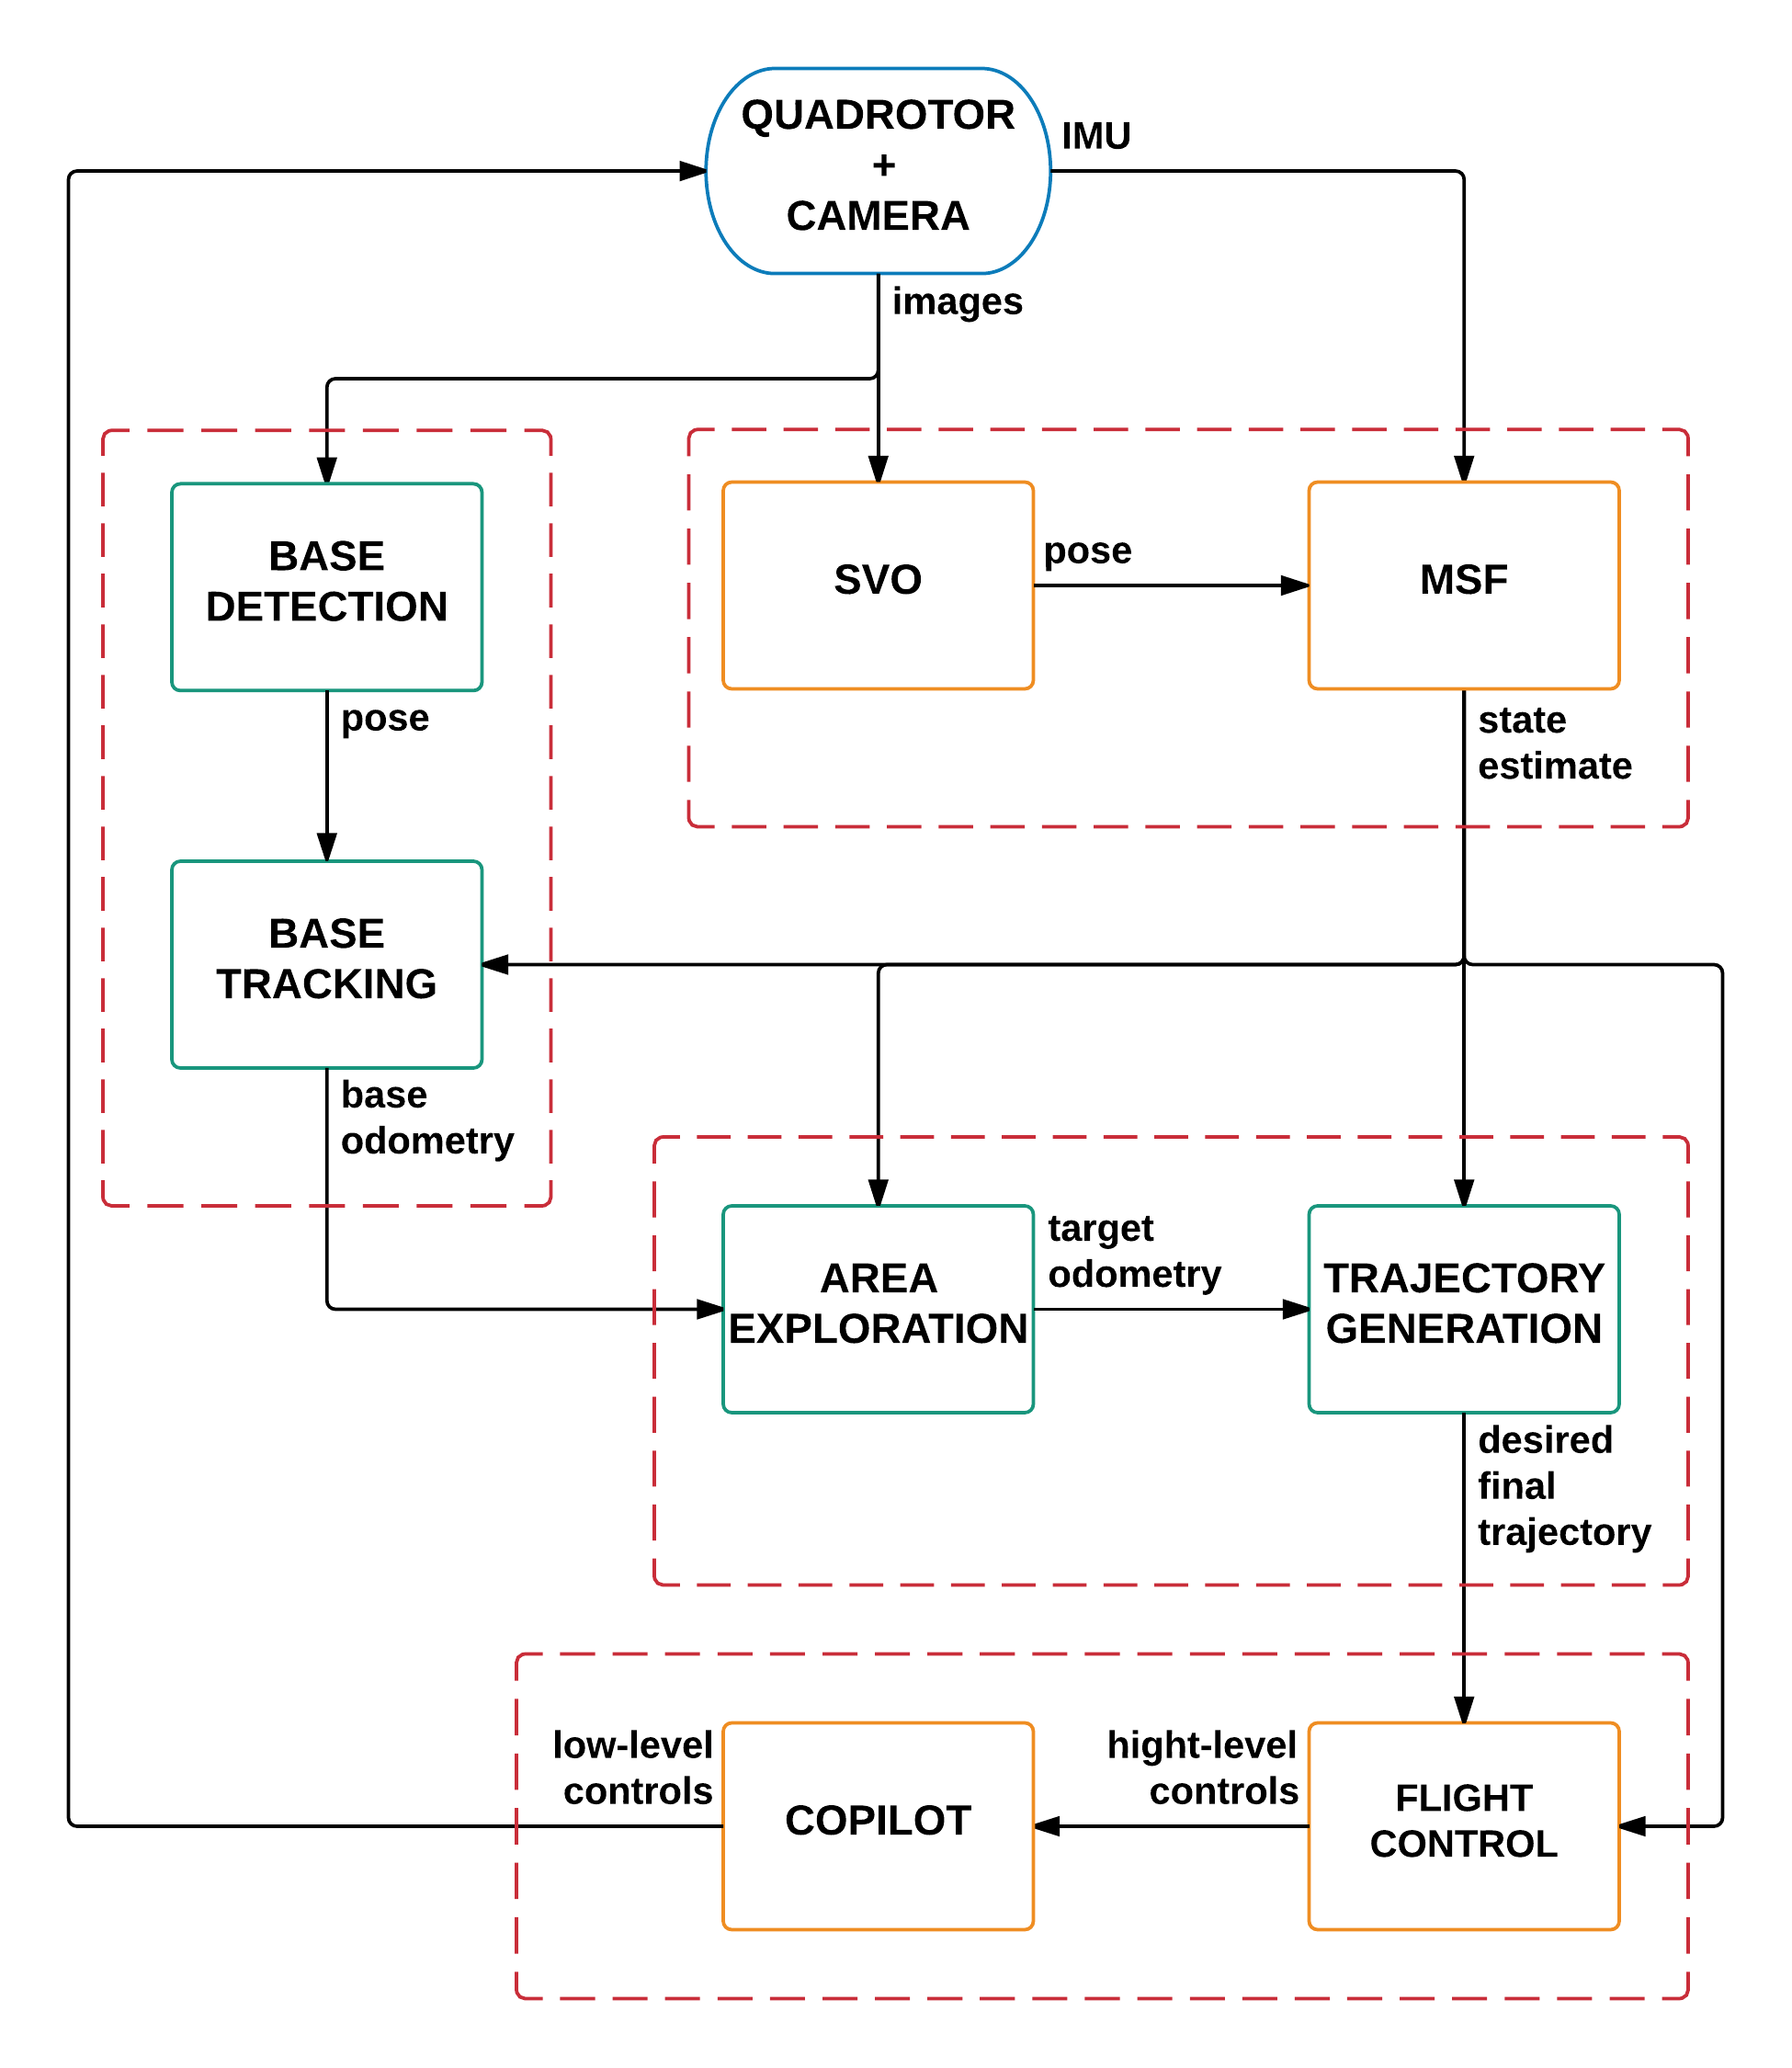
\includegraphics[width=0.97\textwidth]{img/pipeline_diagram.png}
    \caption{Pipeline}
    \label{fig:pipeline_diagram}
\end{figure}

\subsection{SVO \& MSF}
are calculating the best estimation of the state of quadrotor based on data from a camera and an IMU
\subsubsection{SVO front looking camera}
explanation about base in fov\\
Fish eye or not fish eye? pros and cons
\subsection{Base Detection \& Base Tracking}
given images taken from a camera on the quadrotor, it is searching the landing platform and estimating its state
\subsection{Area Exploration \& Trajectory Generation}
considering the state of the quadrotor and of the landing platform, they are calculating where the quadrotor must go and with which trajectory. 

\subsection{Flight Control \& Copilot}
given the desired trajectory, they are computing the controls that must be applied to the quad in order to follow such trajectory
